\documentclass{standalone}
\usepackage{mintikz}

\tikzset{every picture/.style={thick}}

\begin{document}
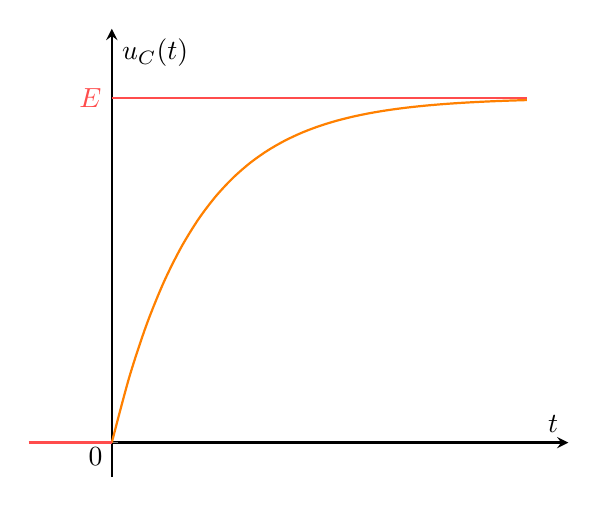
\begin{tikzpicture}[]
    \begin{axis}[
        xmin=-2, xmax=11,
        ymin=-0.5, ymax=6,
        xlabel=$t$, ylabel=$u_C(t)$,
        xtick=\empty, ytick=\empty,
        extra y ticks={0},
        y tick label style={yshift={(\tick==0)*-.5em},
                            xshift={(\tick==0)*.25em}},
        axis lines=center,
        tangent/.style={
            add node at x={#1}{5},
        },
        clip=false]
        \addplot[
            domain=0:10,
            smooth, thick,
            orange]
        {5*(1-exp(-\x/2)};
        \addplot[
            domain=-2:0,
            smooth, thick,
            Red!70]
        {0};
        \addplot[
            domain=0:10,
            smooth, thick,
            Red!70]
        {5} node [pos=0, left] {$E$};
    \end{axis}
\end{tikzpicture}

\end{document}
